\section{担当B — センサ処理・状態機械}

\subsection{機能一覧}

担当Bでは，楽器ユニットにおけるセンサー処理およびArduinoによる制御を担当する．
本システムでは，指揮者ロボットの腕に搭載されたLEDをフォトトランジスタで検出し，
その情報をもとに演奏タイミングを決定する．

各楽器ユニットは独立して動作しており，
通信を用いることなく指揮者の動きに追従して同期演奏を行う．

各楽器ユニットは，あらかじめ内部に楽譜データを保持しており，
取得した拍情報に基づいて順次演奏を行う．
各楽器の演奏開始タイミングは，親機のカラーLEDをカラーセンサで識別することで決定される．
各楽器ユニットはあらかじめ自楽器に対応する色名を設定しており，
その色を拍タイミングで検出した時点で演奏を開始する．

担当Bが提供する主な機能を以下に示す．

\begin{itemize}
  \item フォトトランジスタによる拍タイミングの検出（デジタル入力）
  \item EMA（指数移動平均）によるテンポ推定
  \item カラーセンサによる演奏開始キュー（色）の判別
  \item 状態機械による演奏状態の管理
  \item 担当Cへの拍タイミング・状態情報の共有
\end{itemize}

\subsection{システム構成図}

図\ref{fig:system_B} にシステム全体の構成を示す．

\begin{figure}[H]
\centering
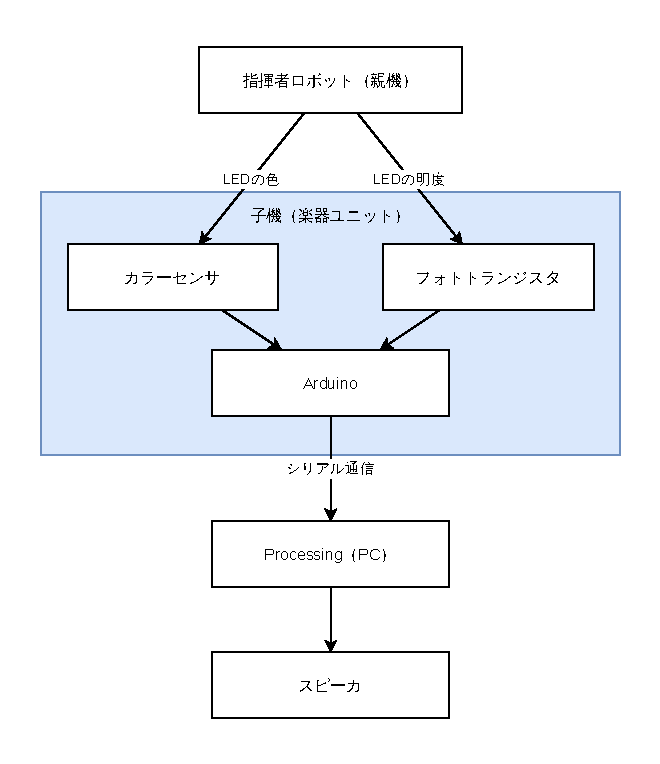
\includegraphics[width=0.8\linewidth]{figures/tantoB/B_system.pdf}
\caption{システム構成図}
\label{fig:system_B}
\end{figure}

\subsection{操作インターフェース設計}

本システムでは，指揮者ロボットの腕の動きが操作インターフェースとなる．
各楽器ユニットはフォトトランジスタとカラーセンサを通じて指揮者の動きを観測することで，
ユーザーが個別の楽器を操作することなく演奏タイミングを制御できる．

\subsubsection*{計測方法}
本システムでは，フォトトランジスタとカラーセンサの2種類のセンサを用いて
指揮者の動きを計測する．
フォトトランジスタにより拍のタイミングを検出し，
カラーセンサにより演奏開始キューの色を判別することで，
各楽器の演奏開始タイミングを決定する．

\subsubsection*{拍の検出（フォトトランジスタ）}
フォトトランジスタは，受光量に応じて出力が変化する素子であり，
デジタルピンから \texttt{HIGH} / \texttt{LOW} を読み取ることで受光量を取得する．
指揮者の腕が振り下ろされた瞬間に点灯するLEDの光を受光すると出力が \texttt{HIGH} に切り替わる．
この立ち上がりエッジを毎ループのポーリングで検出することで拍の基準タイミングを取得する．
チャタリングおよびノイズ誤検出を防ぐため，前回の検出から200\,ms以内の再検知は無視する（300\,BPM相当）．

\subsubsection*{演奏開始キューの判別（カラーセンサ）}
演奏者がProcessing GUIから任意の順序で各楽器を指定することで，
親機のカラーLEDが対応する色を発光する．
カラーセンサ（AE\_S13683\_LED）は拍を検出したタイミングで一発測定を行い，
取得したRGB値をコサイン類似度で色名に変換する（表\ref{tab:detect_colors}）．
各楽器ユニットはあらかじめ自楽器に対応する色名を \texttt{PLAY\_COLOR\_NAME} に設定しており，
検出した色が一致した時点で演奏開始フラグ（\texttt{isPlaying}）を立て，
以降の拍タイミングで楽譜の送信を開始する．

楽器IDとカラーLEDの対応を表\ref{tab:color_map}に示す．

\begin{table}[H]
\centering
\caption{判別対象の色一覧}
\label{tab:detect_colors}
\begin{tabular}{lrrr}
\hline
色名 & 参照R（正規化） & 参照G（正規化） & 参照B（正規化） \\\hline
Red     & 0.975 & 0.222 & 0.017 \\
Green   & 0.130 & 0.957 & 0.261 \\
Blue    & 0.088 & 0.406 & 0.910 \\
Yellow  & 0.524 & 0.828 & 0.203 \\
Cyan    & 0.082 & 0.754 & 0.653 \\
Magenta & 0.519 & 0.371 & 0.770 \\
White   & 0.364 & 0.717 & 0.596 \\\hline
\end{tabular}
\end{table}

\begin{table}[H]
\centering
\caption{楽器IDとカラーLEDの対応（\texttt{PLAY\_COLOR\_NAME} 設定値）}
\label{tab:color_map}
\begin{tabular}{ccc}
\hline
楽器ID & 楽器名 & \texttt{PLAY\_COLOR\_NAME} \\\hline
楽器1 & ハイハット・シンバル & Red（赤） \\
楽器2 & バス・スネア         & Green（緑） \\
楽器3 & 鉄琴                 & Blue（青） \\
楽器4 & ピアノ               & Yellow（黄） \\
楽器5 & トランペット         & White（白） \\\hline
\end{tabular}
\end{table}

\subsubsection*{テンポ推定}
フォトトランジスタによって取得した連続する2拍の検出時刻から
拍間隔$\Delta t_n$を求め，EMAによって拍間隔推定値$T_n$を更新する．

\begin{equation}
  T_n = \alpha \cdot \Delta t_n + (1 - \alpha) \cdot T_{n-1}
\end{equation}

ここで$\alpha$はEMA係数（$0 < \alpha < 1$）であり，$\alpha = 0.2$とする．
測定拍間隔$\Delta t_n$と前回推定拍間隔$T_{n-1}$の誤差率が
閾値$\delta$（デフォルト10\%）を超えた場合はEMAをバイパスして$\Delta t_n$を直接採用し，
急激なテンポ変化に素早く追従する．なお，この誤差率チェックは予備振り状態（PREBEAT）では行わず，
常にEMAを適用する．

\begin{equation}
  \text{誤差率} = \frac{|\Delta t_n - T_{n-1}|}{T_{n-1}} \times 100 \quad [\%]
\end{equation}

次の拍の予測時刻$t_{\text{next}}$は以下の式で計算する．

\begin{equation}
  t_{\text{next}} = t_{\text{beat}} + T_n
\end{equation}

\subsection{状態遷移図}

本システムでは，演奏状態を以下の3状態で管理する．

\begin{itemize}
  \item 停止状態（IDLE）：演奏を行わない状態．電源投入時はこの状態から開始する．
  \item 予備振り状態（PREBEAT）：テンポを確定するために拍を観測する状態．
  \item 通常演奏状態（PLAYING）：EMAによる予測値に基づいて演奏を行う状態．
\end{itemize}

図\ref{fig:state_B} に状態遷移関係を示す．

\begin{figure}[H]
\centering
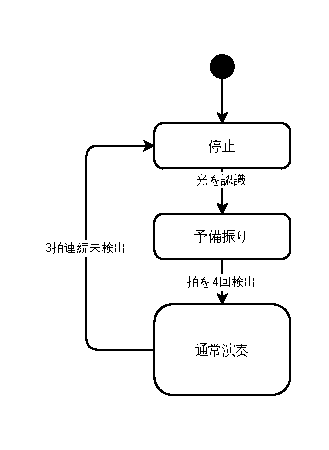
\includegraphics[width=0.8\linewidth]{figures/tantoB/B_state.pdf}
\caption{状態遷移図}
\label{fig:state_B}
\end{figure}

各状態は，センサーから取得した情報に基づいて以下の条件で遷移する．

\begin{itemize}

\item 停止状態 $\rightarrow$ 予備振り状態\\
累積拍検出回数（\texttt{detectCount}）が2以上であり，
かつ現在のループで拍が検出された場合に遷移する．

\item 予備振り状態 $\rightarrow$ 通常演奏状態\\
予備振り中の拍検出回数（\texttt{prebeatCount}）が4回に達した場合に遷移する
（\texttt{PREBEAT\_THRESH = 4}）．

\item 通常演奏状態 $\rightarrow$ 停止状態\\
最後の拍検出から推定拍間隔の3倍以上の時間が経過した場合に遷移する
（\texttt{MISSED\_BEAT\_THRESH = 3}）．

\end{itemize}
